%!TEX root = ../Report.tex
\section{Dialogflow Set-up} % (fold)
\label{sec:dialogflow_setup}
	In IChat, the beta feature ``Knowledge Bases'' is used. So we need to enable it before building the knowledge.

	To simplify the deployment, we use Inline Editor \cite{webhook} (Powered by Cloud Functions for Firebase). It would match a user's query to make suggestions or reply an answer.

	The details would be illustrate in Appendix \ref{cha:user_s_manual} (User's Manual).
% section dialogflow_setup (end)

\section{FAQ Knowledge Test} % (fold)
\label{sec:faq_knowledge_test}
	For Executive Education programs and Stackable Certificate Programs under NUS-ISS website, our team crawled the content from the web page as the knowledge document to build a FAQ document in Dialogflow. However, one question can be phrased into many different ways. If the certain key word are replaced or missing from the question, IChat won’t be able to provide a correct answer. For example, ‘cost’ are trained as the key word for question related to school fees or loans inside the knowledge document. But when user enter word like ‘how much’ or ‘price’, IChat cannot provide the answer related to school fees. Therefore, our team decides to do a knowledge document validation.

	Knowledge document validation is an iterative process and our team focuses on question refinement. For question refinement, different sets of test data is used to run the simulation, and result will be compared with previous iteration to get the highest accuracy rate. Full knowledge document validation question, together with the result are listed in Table \ref{table:faq_test} of Appendix \ref{cha:test_result}.

% section faq_knowledge_test (end)

\section{Intent Test} % (fold)
\label{sec:intent_test}
	For Graduate Programs under NUS-ISS website, our team decide to use intent and fulfillment to represent knowledge to related questions.

	Intent validation is conducted based on the intent we created and training sets we provided in the fulfillment. Different sets of test data is used to run the simulation. Intent details, together with the testing result are appended in Table \ref{table:intent_test} of Appendix \ref{cha:test_result}.
% section intent_test (end)

\section{UI Test} % (fold)
\label{sec:ui_test}
	To get a good user experience, we tested different integration tools \cite{integrations} provided in Dialogflow. The test includes \textbf{Web Demo}, \textbf{Facebook Messenger} and \textbf{Slack}.

	\subsection{Web Demo} % (fold)
	\label{sub:web_demo}
		In the beginning, we wanted to add Web Demo into NUS-ISS website. It successfully replied the user when we said ``hi'' (Figure \ref{fig:web_demo_reply_1}). However, after we had more tests, we realized Web Demo can not reply more than one message and cannot correctly pop up the suggestions we set up in the fulfillment. It only gave the last message showed in Figure \ref{fig:web_demo_reply_2}.

		\begin{figure}[h]
			\centering
			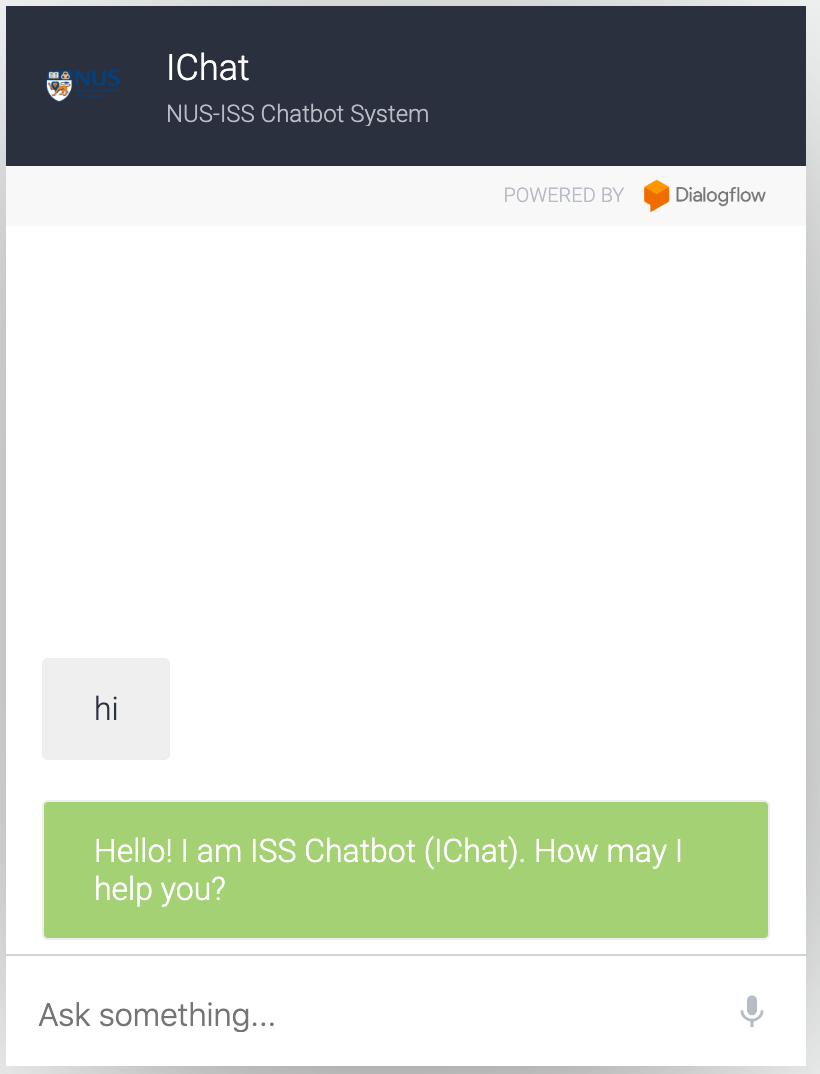
\includegraphics[width=\linewidth/3]{img/webdemo_1.png}
			\caption{Web Demo Reply 1}
			\label{fig:web_demo_reply_1}
		\end{figure}

		\begin{figure}[h]
			\centering
			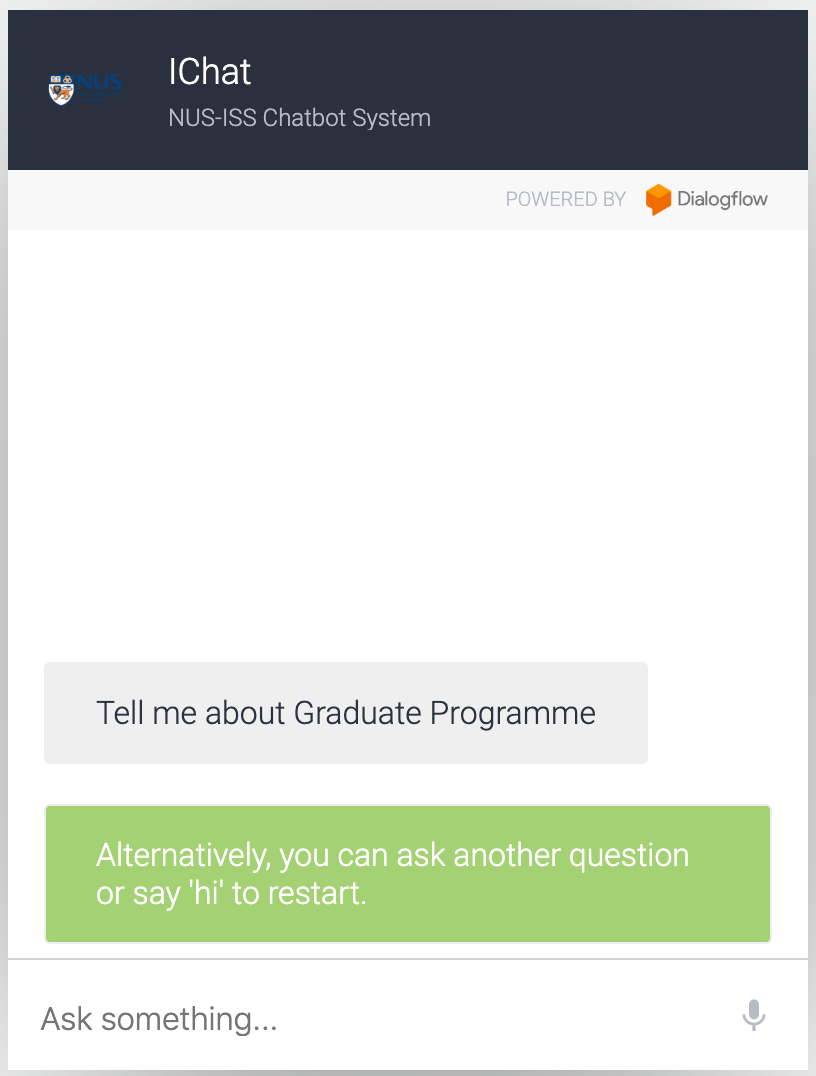
\includegraphics[width=\linewidth/3]{img/webdemo_2.png}
			\caption{Web Demo Reply 2}
			\label{fig:web_demo_reply_2}
		\end{figure}
	% subsection web_demo (end)

	\subsection{Facebook Messenger} % (fold)
	\label{sub:facebook_messenger}
		The Facebook Messenger successfully gave suggestions (Figure \ref{fig:fb_reply_1}) but with one line suggestion which was not very friendly to click if several suggestions were provided. Furthermore, when we clicked the follow-up suggestions, it would cancel the suggestion buttons if the suggestion was not the last message (Figure \ref{fig:fb_reply_2}).

		\begin{figure}[h]
			\centering
			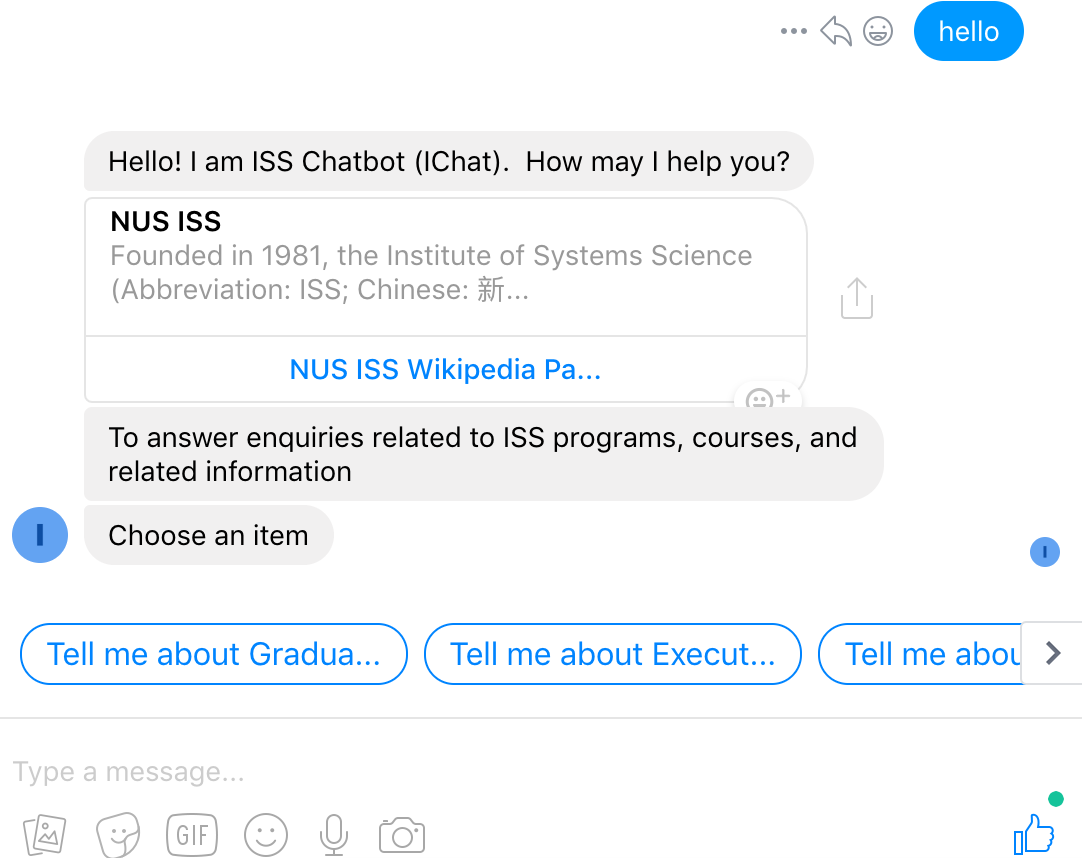
\includegraphics[width=\linewidth/3, frame]{img/fb_1.png}
			\caption{Facebook Messenger Reply 1}
			\label{fig:fb_reply_1}
		\end{figure}

		\begin{figure}[h]
			\centering
			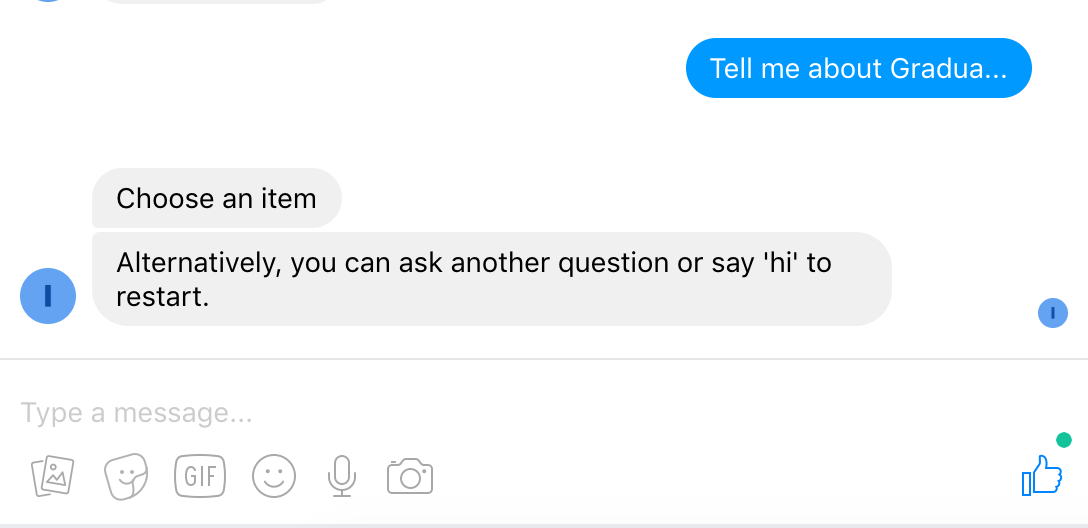
\includegraphics[width=\linewidth/3, frame]{img/fb_2.png}
			\caption{Facebook Messenger Reply 2}
			\label{fig:fb_reply_2}
		\end{figure}
	% subsection facebook_messenger (end)

	\subsection{Slack} % (fold)
	\label{sub:slack}
		At last, we chose Slack which can give a relatively good result (Figure \ref{fig:slack_reply_1}) compared with Web Demo and Facebook Messenger. It gave suggestions and still kept them in the history (Figure \ref{fig:slack_reply_2}) so the user are more flexible to go back choosing other questions. Since Slack can be accessed from different devices, it means the user can enquiry via mobile or desktop.

		\begin{figure}[h]
			\centering
			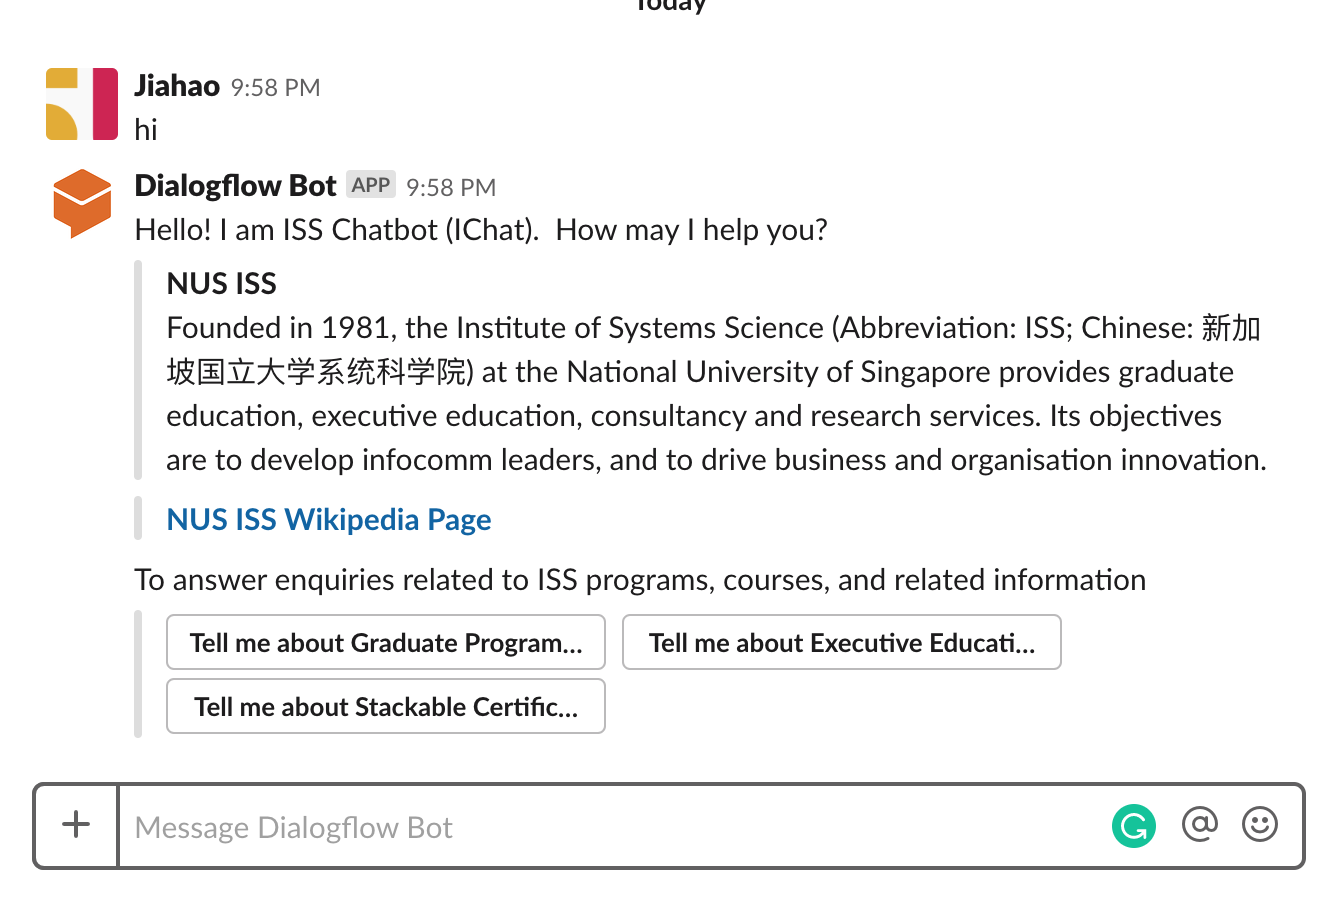
\includegraphics[width=\linewidth/2, frame]{img/slack_1.png}
			\caption{Slack Reply 1}
			\label{fig:slack_reply_1}
		\end{figure}

		\begin{figure}[h]
			\centering
			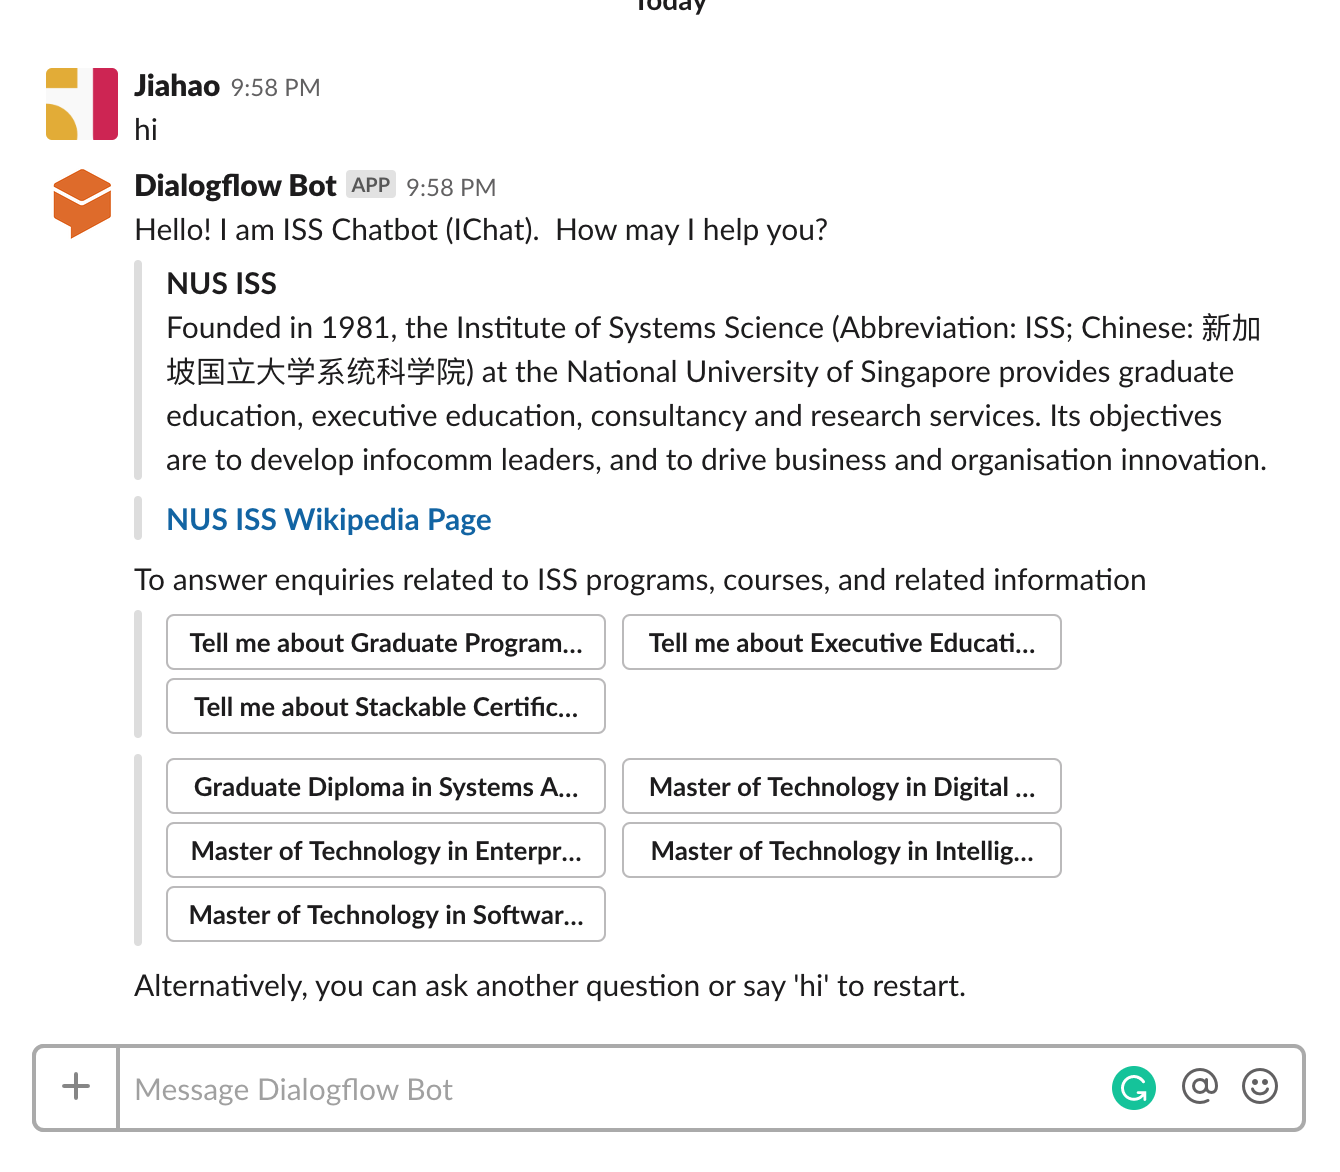
\includegraphics[width=\linewidth/2, frame]{img/slack_2.png}
			\caption{Slack Reply 2}
			\label{fig:slack_reply_2}
		\end{figure}
	% subsection slack (end)

% section ui_test (end)